\section{Policy gradient methods}
\label{sec:policy_learning}
\textit{This section reviews the lecture slides 7, 8, 9 and 10.}
\begin{itemize}
	\item In this section we will discuss techniques for learning the policy directly. There are couple of advantages to it:
	\begin{itemize}
		\item We are able to deal with continuous actions
		\item We are changing the policy \textit{smoothly}, meaning that after an update, we only slightly change the probability distribution over actions. In case of $\epsilon$-greedy on $q$-values, the policy heavily changes when best action becomes another one
		\item Small errors in the value functions don't give a big error in $\pi$ (we are directly optimizing the quantity of interest)
		\item We are able to include prior knowledge, like "don't fall of the cliff", "going left is potentially more interesting", etc.
		\item We are able to learn how much stochasticity is optimal for the given environment. 
	\end{itemize}
	\item In case we have discrete actions, we can simply learn by a softmax over these (viewing them as different classes). For continuous, we can for example use a Gaussian, and learn to predict its mean and variance
	\item The objective of a policy is always the same, namely optimize the expected return for its start state(s): $$J(\theta)=v_{\pi_{\theta}}(s_0)=\E\left[\sum_{t=0}^{T-1} r_{t+1}\right]$$
	Note that we assume here $\gamma=1$. We will use it throughout this section as it makes the derivations/discussion a bit easier, but we can change this term if necessary.
	\item The simplest update is using \textbf{finite difference}, meaning that we estimate the gradients by a small parameter change:
	$$\nabla J(\theta)\approx \frac{ J(\theta+\epsilon) - J(\theta-\epsilon)}{2\epsilon}$$
	However, this means that for $n$ parameters, we would need at least $2n$ roll-outs for an estimate. For stochastic policies, this estimate is extremely noisy and hence, not really applicable.
\end{itemize}
\subsection{REINFORCE and the Policy Gradient Theorem}
\begin{itemize}
	\item The Policy Gradient Theorem says that the gradients of $\nabla_{\theta}J(\theta)$ are proportional to:
	$$\nabla_{\theta}J(\theta) \propto \sum_s \mu(s) \sum_a \nabla_{\theta} \pi_{\theta}(a|s)q_{\pi_{\theta}}(s,a) $$
	Note that we are not interested in the constant proportionality factor because we will absorb it anyways in the learning rate
	\item For deriving the REINFORCE algorithm, we follow the approach of the lecture slides. Let's define $\tau$ as a trajectory that starts from $s_0$ and ends in a arbitrary terminal state. Then, the expected return is the expected return over these trajectories. Using this equality, we can derive the gradients as:
	\begin{equation*}
		\begin{split}
			\nabla_{\theta}J(\theta) & =  \nabla_{\theta} \E_{\tau}[G(\tau)]\\
			& = \int \nabla_{\theta} p_{\theta}(\tau) G(\tau)d\tau\\
		\end{split}
	\end{equation*}
	where the probability of a trajectory is defined as $p_{\theta}(\tau)=p(s_0)\prod_{t=1}^{T}\pi_{\theta}(A_t|S_t)p(S_{t+1}|A_{t},S_t)$, and $G(\tau)$ is the expected return from the initial state. Using the trick $\nabla_{\theta} p_{\theta}(\tau)=p_{\theta}(\tau)\cdot \nabla_{\theta} \ln p_{\theta}(\tau)$, we get:
	
	\begin{equation*}
		\begin{split}
			\nabla_{\theta}J(\theta) & = \int \nabla_{\theta} p_{\theta}(\tau) G(\tau)d\tau\\
			& = \E_{\tau}[G(\tau)\nabla_{\theta} \ln p_{\theta}(\tau)]\\
			& = \E_{\tau}\left[G(\tau)\sum_{t=1}^{T}\nabla_{\theta} \ln p_{\theta}(a_t|s_t)\right]\\
		\end{split}
	\end{equation*}
	\item Hence, to estimate the gradient, we can sample trajectories and approximate the expectation above. This estimate is unbiased but has some disadvantages. The efficiency of REINFORCE is low because of its high variance which comes from two points:
	\begin{itemize}
		\item First, REINFORCE can be seen as a Monte Carlo method of policy-based RL. Hence, the MC samples bring a certain level of noise with them
		\item Suppose we are playing CartPole. Our reward is 1 for each time step, until we terminate. This leads to always positive gradients, which can be seen as "supporting" the last actions. Only if we sample the other action, we might experience an even higher return which pushes the policy towards the newly explored actions. 
	\end{itemize}
	\item The second issue can be tackled by the usage of a \textit{baseline} which is a constant subtracted from the return, that does not influence the gradients being unbiased:
	\begin{equation*}
		\begin{split}
			\E_{\tau}\left[\left(G(\tau)-b\right)\sum_{t=0}^{T}\nabla_{\theta} \ln p_{\theta}(a_t|s_t)\right] & = \E_{\tau}\left[G\left(\tau\right)\sum_{t=0}^{T}\nabla_{\theta} \ln p_{\theta}(a_t|s_t)\right]  - \E_{\tau}\left[b\sum_{t=0}^{T}\nabla_{\theta} \ln p_{\theta}(a_t|s_t)\right] \\
			& = \nabla J(\theta) - b\underbrace{\int p_{\theta}(\tau)\nabla_{\theta} \ln p(\tau)d\tau}_{=0}\\
			& = \nabla J(\theta) 
		\end{split}
	\end{equation*}
	\item A good baseline is the expected reward, which we for example can aggregate over the past.
	\item However, there is one drawback which still remains. We assign each action of a trajectory the same credit, meaning that we punish every action equally no matter how much it actually was responsible for it. This is especially a problem when we punish actions for something in the past (e.g. if last 5 steps get reward of 10 each, but first got -100, we punish all of them equally). To prevent this, we move to G(PO)MDP
\end{itemize}
\subsubsection{G(PO)MDP}
\begin{itemize}
	\item Gradient estimates for (Partially Observable) Markov Decision Processes
	\item Let's reconsider the gradient estimate again, and try to split it into a part before $t$, and a part after $t$:
	
	\begin{equation*}
		\begin{split}
			\nabla_{\theta}J(\theta) & =  \E_{\tau}\left[G(\tau)\sum_{t=1}^{T}\nabla_{\theta} \ln p_{\theta}(a_t|s_t)\right]\\
			& = \E_{\tau}\left[\sum_{t=1}^{T} r_t \sum_{t'=1}^{T}\nabla_{\theta} \ln p_{\theta}(a_{t'}|s_{t'})\right]\hspace{5mm}\text{(Put in definition of return)}\\
			& = \sum_{t=1}^{T} \E_{\tau_{1:t}}\E_{\tau_{t+1:T}}\left[r_t \sum_{t'=1}^{T}\nabla_{\theta} \ln p_{\theta}(a_{t'}|s_{t'})\right]\hspace{5mm}\text{(Move sum out and split expectation)}\\
			& = \sum_{t=1}^{T} \E_{\tau_{1:t}}\left[r_t \left(\sum_{t'=1}^{t}\nabla_{\theta} \ln p_{\theta}(a_{t'}|s_{t'}) + \underbrace{\E_{\tau_{t+1:T}}\left[\sum_{t'=t+1}^{T}\nabla_{\theta} \ln p_{\theta}(a_{t'}|s_{t'})\right]}_{=\E[\int p(x)\nabla\log p(x)dx]=0}\right)\right]\\
			& = \sum_{t=1}^{T} \E_{\tau_{1:t}}\left[r_t \sum_{t'=1}^{t}\nabla_{\theta} \ln p_{\theta}(a_{t'}|s_{t'}) \right]\\
			& = \E_{\tau}\left[\sum_{t=1}^{T}  r_t \sum_{t'=1}^{t}\nabla_{\theta} \ln p_{\theta}(a_{t'}|s_{t'}) \right]
		\end{split}
	\end{equation*}
	With this rewritten gradient, we give credit for $r_t$ only those actions that came \textit{before} $t$
	\item This reduces the variance from REINFORCE, and can be combined with baselines etc. However, keep in mind that we still have a Monte Carlo sample, so that there remains a significant variance
\end{itemize}
\subsubsection{PGPE}
\begin{itemize}
	\item Even when sampling from stochastic policies during a rollout, the variation and exploration we get is mostly fairly limited. Furthermore, we end up with small perturbations (choose "left"-"right"-"left" in CartPole) which are less likely to be repeated by a deterministic policy, and can damage e.g. a robot in real-life situations
	\item Instead, we rather \textit{sample} a deterministic policy $\pi_{\theta}$ from a distribution $p(\theta|\nu)$.  The advantage is that if we now see a state twice, we can guarantee that our policy takes a same action although we are still exploring/stochastic. 
	\item So, instead of choosing $a$ at every randomly, we randomly choose the action for any state in the beginning (represented by $\pi_{\theta}$), and keep it fixed over the trajectory
	\item Our gradient (which is now with respect to $\nu$ as we want to learn $p(\theta|\nu)$) is:
	$$\nabla_{\nu} J(\nu) = \E_{\theta}\E_{\tau|\pi_{\theta}}[G(\tau) \nabla_{\nu}p(\theta;\nu)]$$
\end{itemize}
\subsection{Actor-critic Policy Gradient}
\begin{itemize}
	\item Although we increased the stability of REINFORCE by the discussed improvements, the problems of Monte Carlo sampling remain: we have to wait until the end of the episode, and the samples have a high variance
	\item First we take a look again at G(PO)MDP, where we slightly re-arrange the terms:
	$$\E_{\tau}\left[\sum_{t=1}^{T}  r_t \sum_{t'=1}^{t}\nabla_{\theta} \ln p_{\theta}(a_{t'}|s_{t'}) \right] = \E_{\tau}\left[\sum_{t'=1}^{T}\nabla_{\theta} \ln p_{\theta}(a_{t'}|s_{t'}) \sum_{t=t'}^{T}  r_t\right]$$
	In our value-based methods, we previously learn the terms $\sum_{t=t'}^{T}  r_t$ by the $v$/$q$-functions, as it is the expected value of those. Hence, we can also plug them in here:
	$$\E_{\tau}\left[\sum_{t'=1}^{T}\nabla_{\theta} \ln p_{\theta}(a_{t'}|s_{t'}) \sum_{t=t'}^{T}  r_t\right] = \E_{\tau}\left[\sum_{t'=1}^{T}\nabla_{\theta} \ln p_{\theta}(a_{t'}|s_{t'}) q_{\pi}(s_{t'},a_{t'})\right]$$
	\item The question arises whether we can replace $q_{\pi}(s_{t'},a_{t'})$ by an estimate $\hat{q}_{\bm{w}}(s_{t'},a_{t'})$ without introducing a bias. The answer is yes, but with two constraints on the function $\hat{q}_{\bm{w}}$:
	\begin{enumerate}
		\item The function has to be \textit{compatible}, which means:
		$$\nabla_{\bm{w}}\hat{q}_{\bm{w}}(s,a) = \nabla_{\theta}\ln \pi_{\theta}(a|s)\hspace{5mm}\text{like}\hspace{2mm} \hat{q}_{\bm{w}}(s,a)=\bm{w}^T \nabla_{\theta} \ln \pi_{\theta}(a|s)$$
		\item $\hat{q}_{\bm{w}}$ has to be fully converged, i.e.
		$$\E\left[(q_{\pi}(s,a)-q_{\bm{w}}(s,a)) \frac{\partial \hat{q}_{\bm{w}}(s,a)}{\partial \bm{w}}\right]= 0$$
	\end{enumerate}
	\item We call the policy $\pi$ the actor, while $\hat{q}_{\bm{w}}$ is the critic
	\item Note that we can still add a baseline to stabilize learning further. For example, a good baseline is the value function so that our actual goal of $\hat{q}_{\bm{w}}$ should be to learn $\hat{q}_{\bm{w}}(s,a)\approx q_{\pi}(s,a)-v_{\pi}(s)=A(s,a)$ which is also called the \textbf{advantage}
	\item The \underline{benefits} of actor-critic methods is a lower variance as the target is not sampled anymore, and we can update our policy more frequently instead of waiting until the end of the episode.
	
	However, the \underline{drawbacks} are that we have more hyperparameters to finetune (two learning rates etc.), and we require an stochastic policy (no full greedy policy possible). We will see later methods which can deal with deterministic ones.
\end{itemize}
\subsubsection{Generalized Advantage Estimation (n-step AC)}
\begin{itemize}
	\item Let's reconsider the difference between actor-critic and actor-only approaches from a different perspective. Actor-critic bootstrap its estimate on the next value, which is very similar to TD(0) learning. Actor-only uses the sampled return, which is a Monte Carlo method. In value-based methods, we discussed that we can generalize TD(0) and Monte Carlo to $n$-step TD learning which we can do here similarly. This is again a trade-off between variance and bias. %  because as we have seen before, if $\hat{q}_{\bm{w}}$ has not fully converged (which is in practice mostly not the case), we get a biased estimate of our gradients.
	\item The advantage for an $n$-step estimate is:
	$$\hat{A}_t^n = r_t + \gamma r_{t+1} + ... + \gamma^n v(s_{t+n}) - v(s_t)$$
	where $\delta_{t}$ is the TD error for time step $t$. If $\gamma=1$, we can rewrite it in terms of TD errors: $\hat{A}_t^n = \sum_{l=0}^{n-1}\delta_{t+l}$
	 
	However, we can also take a smoother version of $n$-step, where we take a weighted average of all the advantages:
	$$\hat{A}_t^{GAE} = (1-\lambda)\left(\hat{A}_t^{(1)} + \lambda \hat{A}_t^{(2)} + \lambda^2 \hat{A}_t^{(2)} + ...\right) = \sum_{l=0}^{\infty} (\gamma \lambda)^{l}\delta_{t+l}$$
	which is also known as TD($\lambda$).
	\item A lower $\lambda$ reduces the variance but increases the bias (TD). Similarly, choosing a high $\lambda$ gives a low bias but high variance (MC).
	
	However, a disadvantage of using $\lambda$ instead of a fixed $n$ is that we need to run a full episode before we can calculate any advantage.
	\item This approach can again be used in combination with many different optimization techniques, like using TRPO (see next section). 
\end{itemize}
\subsection{Higher-order Policy Search Methods}
\begin{itemize}
	\item When updating our policy, we want to make sure that we don't change too much. The reason for that is that our samples come from $\pi_{\theta}$. The more we change $\pi_{\theta}$, the more our gradient estimate becomes inaccurate! Hence, we should limit our change in $\pi_{\theta}$.
	\item A simple way of checking that is by taking the L2 norm over parameters, namely $d\theta^T d\theta$, and fix this norm to a certain value $c$
	\item To find the next optimal value, we have to solve the following equation for the step we take, namely $\theta^{*}-\theta_0$ ($\theta^{*}$ next value), such that $d\theta^T d\theta=c$:
	\begin{equation*}
		\begin{split}
			\theta^{*}-\theta_0 & = \max_{d\theta} J(\theta_0 + d\theta)\\
			& \approx \max_{d\theta} J(\theta_0) + (\nabla_{\theta} J(\theta))^T d\theta \hspace{5mm}\text{(Taylor expansion)}\\
			& \propto \nabla_{\theta} J(\theta)
		\end{split}
	\end{equation*}
	This means that the previous, standard policy gradient methods maximize the Taylor expansion of $J$ such that the update is on the norm sphere (as $d\theta^T d\theta=c$)
	\item However, there are many disadvantages and possible problems of this:
	\begin{itemize}
		\item The norm itself is highly sensitive to the parameterization of the model. For example, consider a Gaussian for which we want to learn the mean and the variance. We can achieve the same if we learn the standard deviation, or even the precision of the Gaussian. However, all these parameters have a different scale, and euclidean distance is not always the best distance measurement (e.g. $\sigma=0.1$ and $\sigma=0.2$ are more \textit{different} than $\sigma=10.1$ and $\sigma=10.2$)
		\item Another simple fail case is when we change the scale of the parameters. Suppose we express the mean by $\mu=4\cdot \theta_1$ instead of $\mu=\theta_1$, while keeping $\sigma=\theta_2$. As we only look at the gradient norm of $\theta_1$ and not $\mu$, we take in the first case a four-times as big step than in the other case. This is clearly not desired because both parameterizations express the same model, with just different scales. Furthermore, this can lead to an issue for $\sigma=\theta_2$ as we do not change $\sigma$ equally.
		\item Furthermore, we ignore correlations between parameters. If the gradient of $\theta_1$ and $\theta_2$ are highly correlated, like if we would use $\mu=\theta_1+\theta_2$, we update both as if they were independent.
	\end{itemize}
	\item So, we are not directly interested in the change of the parameters, but of the policy distribution. A better way of doing so is by using the KL divergence as difference:
	$$D_{\text{KL}}(p||q)=\int p(x)\log\frac{p(x)}{q(x)}dx$$
	There are different algorithms that exploits this property, and we will discuss two of them: Natural Policy Gradient, and Trust region policy optimization
\end{itemize}
\subsubsection{Natural Policy Gradients}
\begin{itemize}
	\item The first step for using the KL divergence as step size regulator, is by replacing the constant $c$ by the quadratic expansion of expected KL divergence over states:
	\begin{equation*}
		\begin{split}
			c & = \E_{s}\left[D_{KL}\left(\pi(a|s;\theta_0)||\pi(a|s;\theta)\right)\right] = \text{EKL}(\theta)\\
			& \approx \underbrace{\text{EKL}(\theta_0)}_{=KL(p||p)=0} + d\theta^T \underbrace{(\nabla_{d\theta}\text{EKL})(\theta_0)}_{=0 \text{ as }\theta_0\text{ optimum}} + \frac{1}{2}d\theta^T (\nabla_{d\theta}^2\text{EKL})(\theta_0)d\theta\\
			& = \frac{1}{2}d\theta^T (\nabla_{d\theta}^2\text{EKL})(\theta_0)d\theta\\
		\end{split}
	\end{equation*}
	\item So, to obtain the optimal parameter $c$, we need ot calculate the Hessian $\nabla_{d\theta}^2\text{EKL}$ at point $\theta_0$. This is also known as the Fisher information matrix (i.e. how much information does $\pi$ is changed by $\theta$), and can be calculated by:
	\begin{equation*}
		\begin{split}
			F & = \nabla_{d\theta}^2\text{EKL} = \E_{s}\left[\nabla_{d\theta}^2 D_{KL}\left(\pi(a|s;\theta_0)||\pi(a|s;\theta)\right)\right]\\
			\nabla_{d\theta}^2 D_{KL} & = \E_{a\sim\pi(a|s;\theta_0)}[\nabla_{d\theta}^2 \log \pi(a|s;\theta_0+d\theta)]\\[10pt]
		\end{split}
	\end{equation*}
	$$\implies F = \begin{bmatrix}
	\E_a\left[\nabla_{d\theta_1} \log \pi_{\theta}(a|s)\right]^2 & \E_a\left[\nabla_{d\theta_1} \log \pi_{\theta}(a|s)\right]\cdot \E_a\left[\nabla_{d\theta_2} \log \pi_{\theta}(a|s)\right] & ...\\
	\E_a\left[\nabla_{d\theta_2} \log \pi_{\theta}(a|s)\right]\cdot \E_a\left[\nabla_{d\theta_1} \log \pi_{\theta}(a|s)\right] & \E_a\left[\nabla_{d\theta_2} \log \pi_{\theta}(a|s)\right]^2 & ...\\
	% \E_a\left[\nabla_{d\theta_1} \log \pi_{\theta}(a|s)\right]\cdot \E_a\left[\nabla_{d\theta_3} \log \pi_{\theta}(a|s)\right] & \E_a\left[\nabla_{d\theta_2} \log \pi_{\theta}(a|s)\right]\cdot \E_a\left[\nabla_{d\theta_3} \log \pi_{\theta}(a|s)\right] & ...\\
	\vdots & \vdots & \ddots
	\end{bmatrix}$$
	
	\item Now, we reconsider our update step:
	\begin{equation*}
		\begin{split}
			\theta^{*}-\theta_0 & \approx \max_{d\theta} J(\theta_0) + (\nabla_{\theta} J(\theta))^T d\theta \hspace{5mm}\text{(Taylor expansion)}\\
		\end{split}
	\end{equation*}
	To take the maximum, we now also need to consider our constraint as Lagrangian:
	$$\max_{d\theta}\min_{\lambda} J(\theta_0) + (\nabla_{\theta} J(\theta))^T d\theta + \lambda (d\theta F d\theta-c)$$
	So that, when we solve it, we get:
	$$d\theta  \propto F^{-1}\nabla_{\theta}J(\theta)$$
	which we call the \textit{natural gradient}
	\item The update rule is now:
	$$\theta_{t+1} = \theta_t + \alpha F^{-1}\nabla_{\theta_t}J(\theta_t)$$
	where for the vanilla gradient $\nabla_{\theta_t}J(\theta_t)$, we can use any of the above methods.
	\item We can show that for a sufficiently small step size, we will always improve by this update step 
	\item Figure~\ref{fig:rl_policy_gradients_NPG} shows a visualization of the update difference between NPG and standard policy gradients. NPG allows us to find a better fit in the region of "safe" changes, so that we possibly can take larger steps, towards the right policy.
	
	\begin{figure}[ht!]
		\centering
		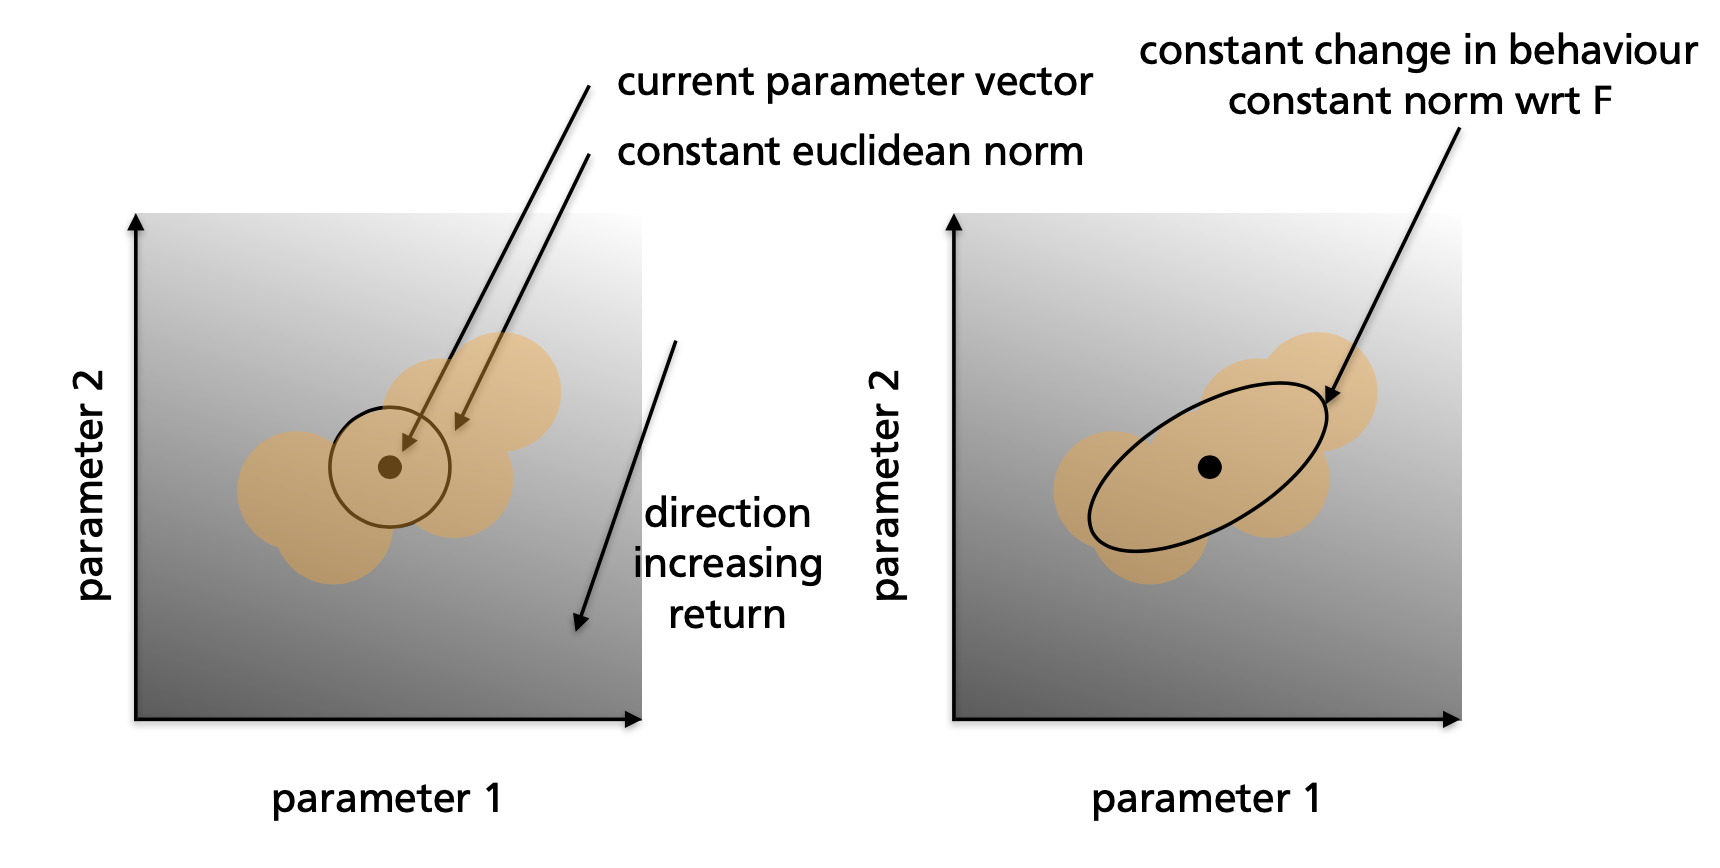
\includegraphics[width=0.5\textwidth]{figures/rl_policy_gradients_NPG.png}
		\caption{Comparison of L2 norm update (left) and NPG (right). The orange background represents the safe changes, meaning the parameter changes for which our policy does not change greater than our defined threshold. While the L2 sticks with the unit sphere, NPG can represents ellipsoids so that we can take larger steps in parameter space towards increasing $J$ without changing the policy too much.}
		\label{fig:rl_policy_gradients_NPG}
	\end{figure}

	We can also visualize the gradient direction grid, as in Figure~\ref{fig:rl_policy_gradients_NPG_gradient_example}. Gradients that point in the wrong direction, give very slow convergence because we focus on parameters which are already close to optimal. 
	
	\begin{figure}[ht!]
		\centering
		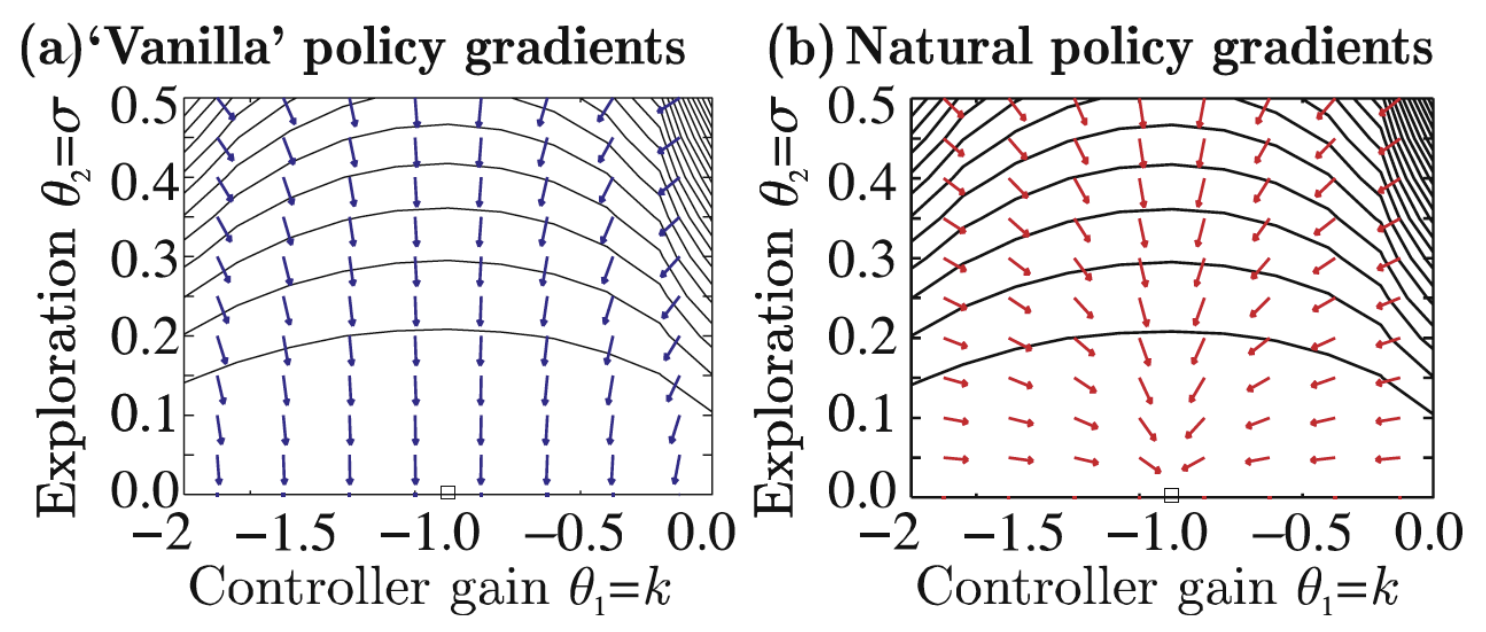
\includegraphics[width=0.4\textwidth]{figures/rl_policy_gradients_NPG_gradient_example.png}
		\caption{Gradient direction over parameter space for finding the optimum at $(-1,0)$. While the NPG gives very smooth transitions, vanilla gradients point straight down (strong gradient for $\theta_2$) for points like $(-2,0.1)$ where we clearly need to update $\theta_1$ more. This leads to slow convergence.}
		\label{fig:rl_policy_gradients_NPG_gradient_example}
	\end{figure}
	\item The advantages of NPG are therefore:
	\begin{itemize}
		\item Faster convergence and less training time
		\item Is an adaptation on top of standard policy gradient, so we can use any of the previous methods with all additions/tricks we want
	\end{itemize}
	However, the biggest drawback is that we have to calculate the Fisher information matrix, which is known for standard distributions like Gaussians, but might be harder to determine for other cases, especially if we want to use a neural network (can be approximated with conjugate gradient algorithm). It also keeps the disadvantages of the other policy gradient methods, namely high variance and namely still slower convergence compared to value-based methods.
\end{itemize}
\subsubsection{Trust region policy optimization}
\begin{itemize}
	\item A problem of Natural Policy Gradient is that we approximated the KL divergence by a second-order Taylor expansion. The errors that we introduced there, might cause our initial KL constraint to break meaning that $d\theta^T F d\theta\neq c$
	\item TRPO takes a bit different view on the problem. The main concept of the algorithm is that we take as big steps as long as we can guarantee improvement. Hence, we have three steps:
	\begin{enumerate}
		\item Approximate the return function $J$
		\item Apply a penalty term to yield lower bound on the exact function
		\item Maximize lower bound (which guarantees improvement on exact function) by e.g. SGD again
	\end{enumerate} 
	\item The region where we assume our approximation to be valid, is called \textit{trust region}
	\item Figure~\ref{fig:rl_policy_gradients_TRPO_vs_NPG} compares the ideas of NPG and TRPO visually. NPG takes a linear approximation of $J$ at a point, and limits the step size by approximating the KL divergence. TRPO however designs a lower bound which is strictly lower than the "true" function. It is a combination of an approximation of $J$, and a penalty term for big chances in the policy 
	\begin{figure}[ht!]
		\centering
		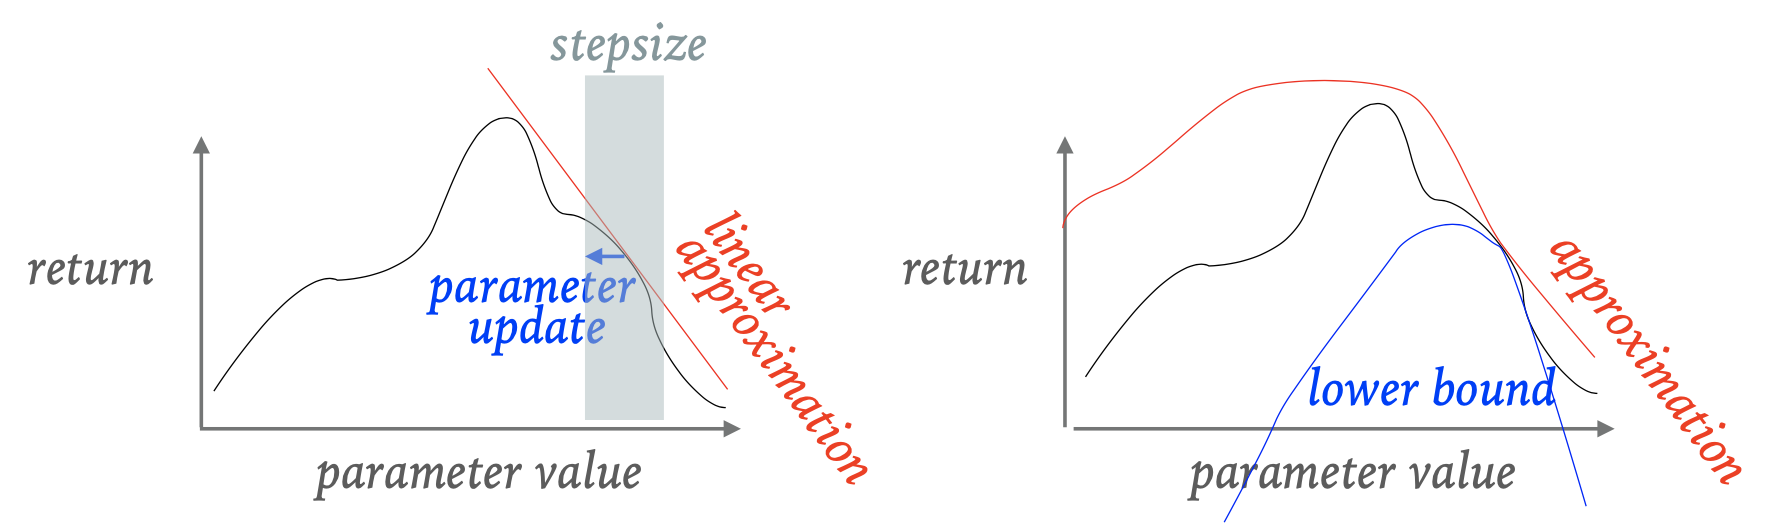
\includegraphics[width=0.55\textwidth]{figures/rl_policy_gradients_TRPO_vs_NPG.png}
		\caption{Comparing the optimization properties of NPG (left) and TRPO (right).}
		\label{fig:rl_policy_gradients_TRPO_vs_NPG}
	\end{figure}
	\item We can calculate the return by:
	$$\eta(\theta)=\E_{\bm{s}\sim \mu_{\pi_{\theta},\bm{a}\sim \pi_{\theta} }(s)}[r(\bm{s},\bm{a})]$$
	where we use samples from $\pi_{\theta}$ to approximate the expectation. However, as soon as we shift $\theta$, we cannot use the same samples anymore because we would be biased. Hence, we can use importance weights:
	$$\eta(\theta)\approx \E_{\bm{s}\sim \mu_{\pi_{\theta}},\bm{a}\sim \pi_{\theta'} (\bm{s})}\left[\frac{\pi_{\theta}(\bm{a}|\bm{s})}{\pi_{\theta'}(\bm{a}|\bm{s})}r(\bm{s},\bm{a})\Bigg\vert \theta' \right]=L_{\theta'}(\theta)$$
	but note that the state distribution is not changed (hence approximation!).
	\item Now, let's consider how we get the lower bound based on our approximation. 
	$$\eta(\theta)\geq L_{\theta'}(\theta) - \frac{2\epsilon \gamma}{(1-\gamma)^2}\cdot \max_s D_{\text{KL}}\left(\pi_{\theta}(\cdot|s)||\pi_{\theta'}(\cdot|s)\right)$$
	where the factor in front of the penalty is environment/policy dependent. 
	\item Although this term above guarantees us a lower bound, in practice, we might run into multiple issues:
	\begin{itemize}
		\item We need to take the maximum KL divergence over all states. However, in environments with many and/or continuous states, this is often not possible. So, we approximate it by taking the average instead.
		\item The penalty is usually very high so that we cannot make big steps. So, the average can already help to reduce the penalty, but we can also consider the KL divergence rather as a constraint than a penalty. This leads us to a similar approach as for NPG
	\end{itemize}
	\item So, what we do instead is maximizing the approximation as in Natural Policy Gradient, but dynamically set the step size based on a maximum KL divergence that we allow between policies. Meaning, we solve the following equation for step size $\beta$:
	$$D_{\text{KL}} \approx \beta^2 d\theta^T F_s d\theta / 2$$
	with $d\theta$ being in the same direction as NPG. One way of (approximately) solving it is by starting with an initial $\beta_0$, and for a couple of steps, increase it if constraint is fulfilled. Otherwise, reduce until we find a valid, sufficiently high $\beta$.
	
	\item In Figure~\ref{fig:rl_policy_gradients_TRPO_vs_NPG}, we now are at the left image again but the step size is adjusted by the KL.
	\item The advantage of TRPO is that we can take bigger steps than the standard NPG, while in theory, having the guarantee of converging. It has been shown to work well with neural controllers where we approximate $F$ by the conjugate gradients. 
	
	The disadvantages are however, that it still requires many steps, and the return is still a Monte Carlo sample (high variance). The guarantee of convergence is actually broken by all the approximations we took.
\end{itemize}

\subsection{Deep Policy Search}
\begin{itemize}
	\item When using deep neural networks for policy search, we might need to consider a few additional tricks because of the high non-linearity of the networks.
	\item To discuss this, we take deterministic policy gradient as an example, and explain the tricks that are used here
\end{itemize}
\subsubsection{Deterministic policy gradients}
\begin{itemize}
	\item All policy gradient methods we have discussed so far considered stochastic policy. However, it is sometimes preferred to learn a deterministic policy (e.g. remember Q-learning)
	\item This means that we will also learn off-policy (behavior policy $b$ with target/actor $\pi$). All other methods were discussed from the on-policy perspective but could be adjusted for off-policy with some minor modifications like importance sampling
	\item When using a different policy for sampling, we change our state distribution from $\mu_{\pi}$ to $\mu_{\beta}$, so that our return is:
	$$J_{\beta}(\pi_{\theta}) = \int_{\mathcal{S}} \mu^{\beta}(s)Q^{\pi}\left(s,\pi_{\theta}(s)\right)ds$$
	In terms of gradients, we end up with:
	$$\nabla_{\theta} J_{\beta}(\pi_{\theta})=\E_{s\sim\mu_{\beta}}\left[\nabla_{\theta}\pi_{\theta}(s)\nabla_a Q^{\pi}(s,a)|a=\pi_{\theta}(s)\right] $$
	Note that this requires $\pi_{\theta}(s)$ to be differentiable, hence returning continuous actions.
	
	Although our samples are slightly off/biased ($\mu_{\beta}$ instead of $\mu_{\pi}$), this is usually not a problem as $\beta$ is chosen to be $\pi$ with some additional noise (like Gaussian).
	\item Our update equations are as follows:
	\begin{equation*}
		\begin{split}
			\text{TD error }\hspace{2mm}\delta_t & = r_t + \gamma Q^{w}\left(s_{t+1}, \pi_{\theta}\left(s_{t+1}\right)\right) - Q^{w}\left(s_{t}, a_t\right)\\
			\text{Update of $Q$ }\hspace{2mm}w_{t+1} & = w_{t} + \alpha_{w}\delta_t \nabla_{w} Q^{w}(s_t,a_t)\\
			\text{Update of $\pi$ }\hspace{2mm}\theta_{t+1} & = \theta_{t} + \alpha_{\theta} \nabla_{\theta} \pi_{\theta}(s_t) \nabla_{a} Q^{w}(s_t,a_t)|_{a=\pi_{\theta}(s)}
		\end{split}
	\end{equation*}
	where we illustrate the gradients in Figure~\ref{fig:rl_policy_gradients_DPG}.
	\begin{figure}[ht!]
		\centering
		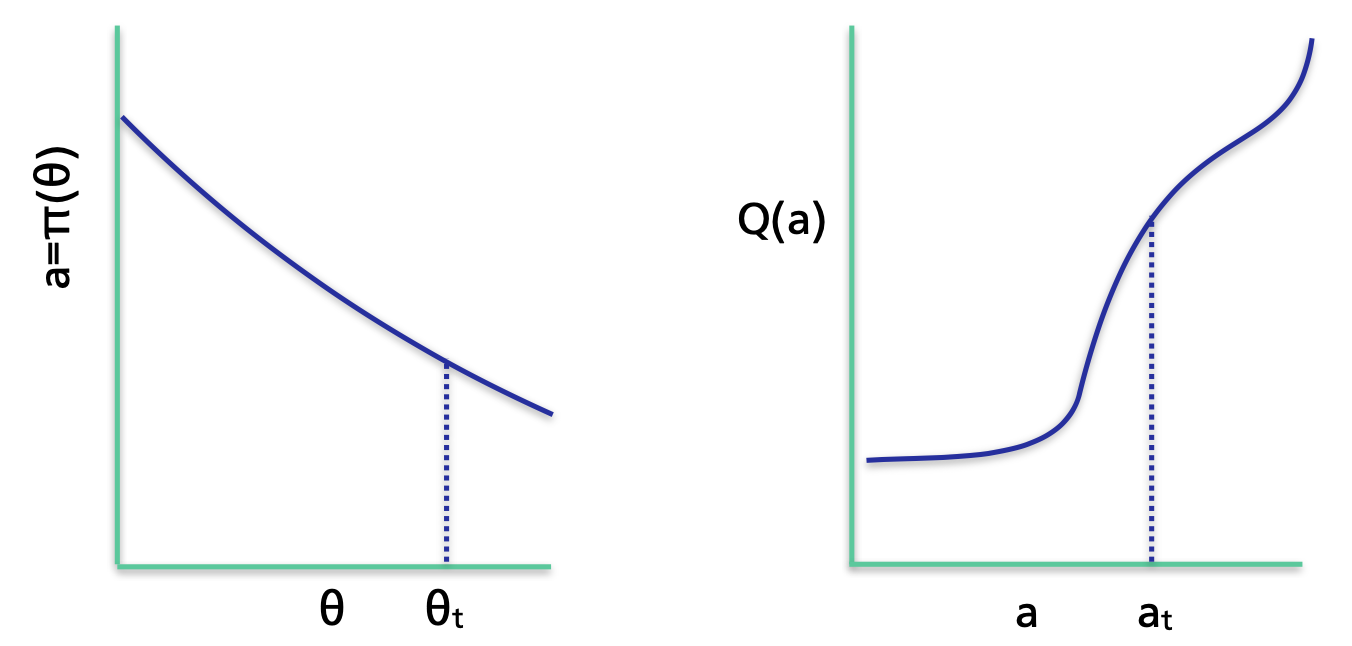
\includegraphics[width=0.5\textwidth]{figures/rl_policy_gradients_DPG.png}
		\caption{Illustrating the gradients in DPG. We have the combination of how much we change the action by changing $\theta$, and how this action change influences the action value $Q^{\pi}$.}
		\label{fig:rl_policy_gradients_DPG}
	\end{figure}
\end{itemize}
\subsubsection{Deep DPG}
\begin{itemize}
	\item When using neural networks, we again have to consider the same issues as in the DQN approach
	\item To use the collected data more efficiently and break the dependency between elements in a batch, we apply \textit{experience replay}
	\item For stabilizing the TD updates, we don't fix the target network, but create a second one that slowly tracks the learned $Q$ values
	\item For ensuring a similar scale of features, we apply \textit{batch normalization} within the network
	\item One aspect of exploration that we have discussed in PGPE before is that independent noise on the actions do not explore well. As a simple improvement, the Deep DPG paper correlates the noise by endorsing to use the same random decision as the time step before
\end{itemize}
\subsection{Summary}
\begin{itemize}
	\item To wrap up policy-based reinforcement learning, we want to put all discussed algorithms into perspective.
	
	\begin{figure}[ht!]
		\centering
		\begin{subfigure}{0.45\textwidth}
			\centering
			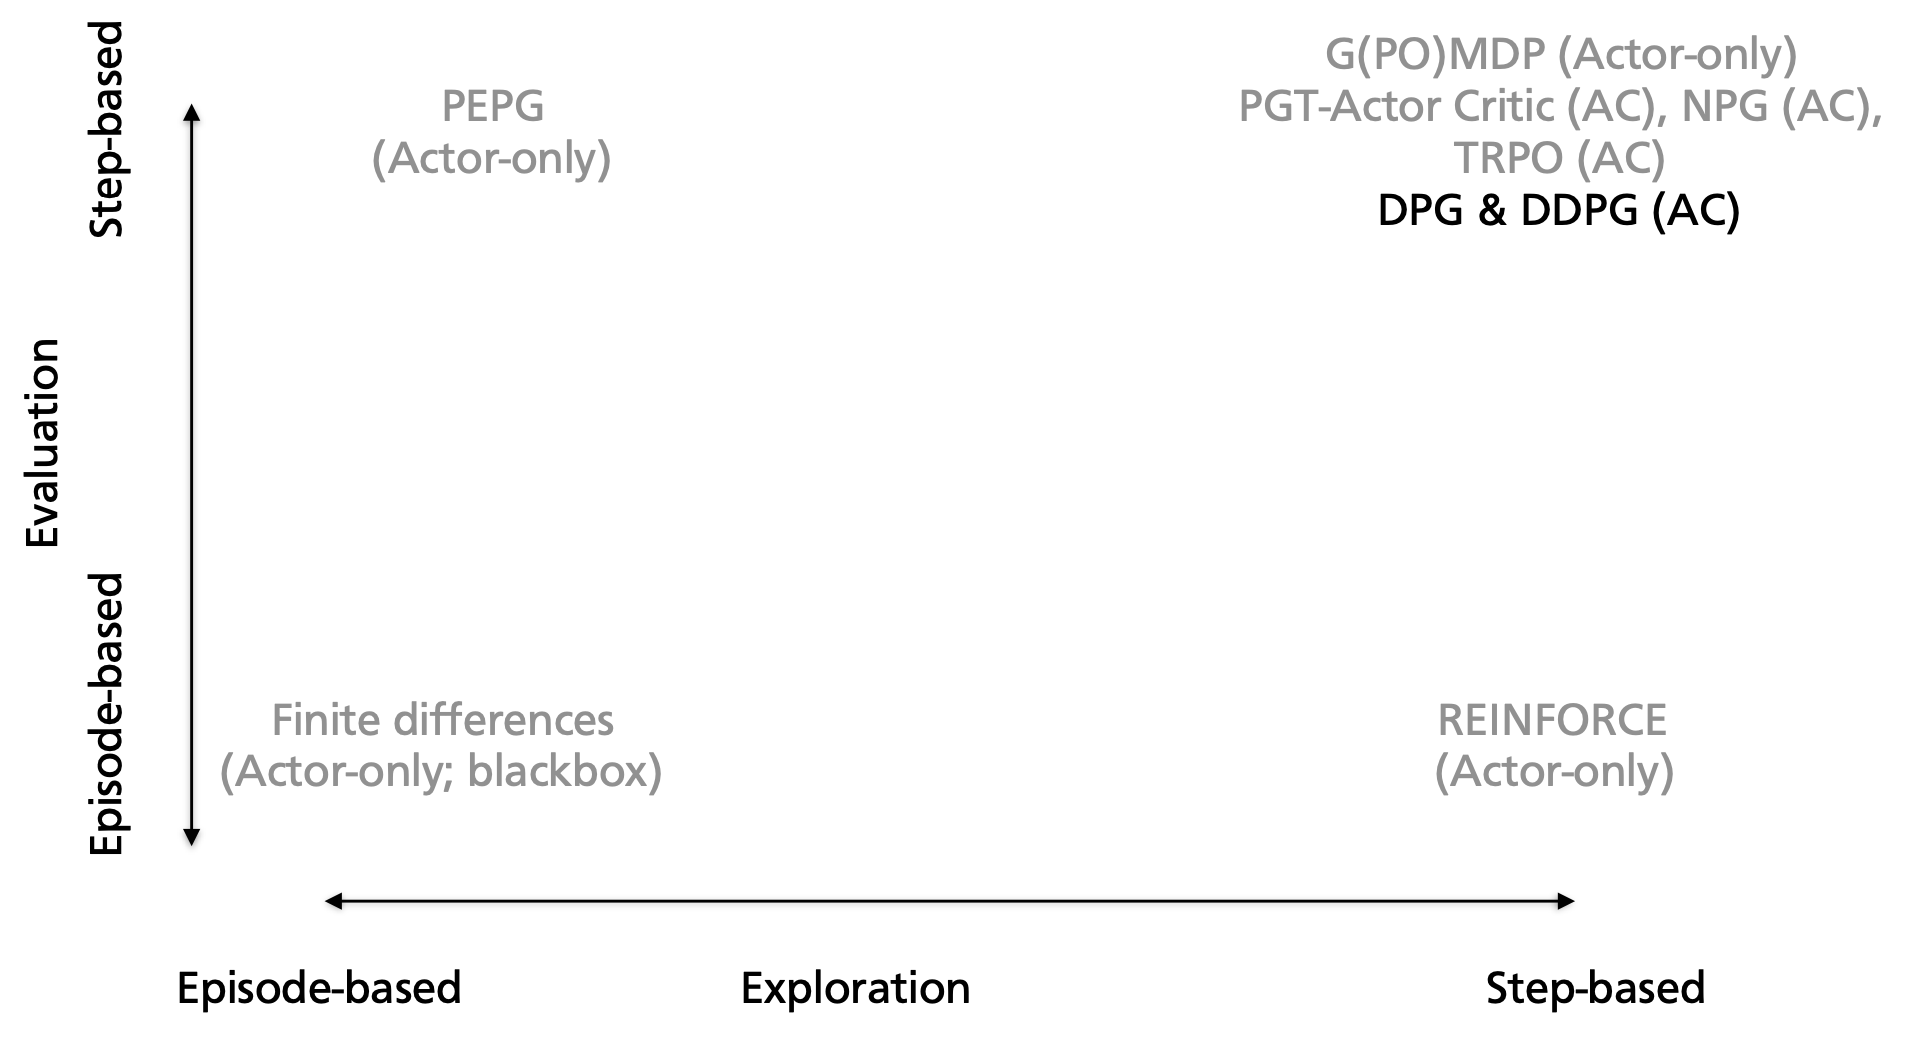
\includegraphics[width=\textwidth]{figures/rl_policy_gradient_summary_1.png}
			\caption{Exploration vs Evaluation}
		\end{subfigure}
		\hspace{5mm}
		\begin{subfigure}{0.45\textwidth}
			\centering
			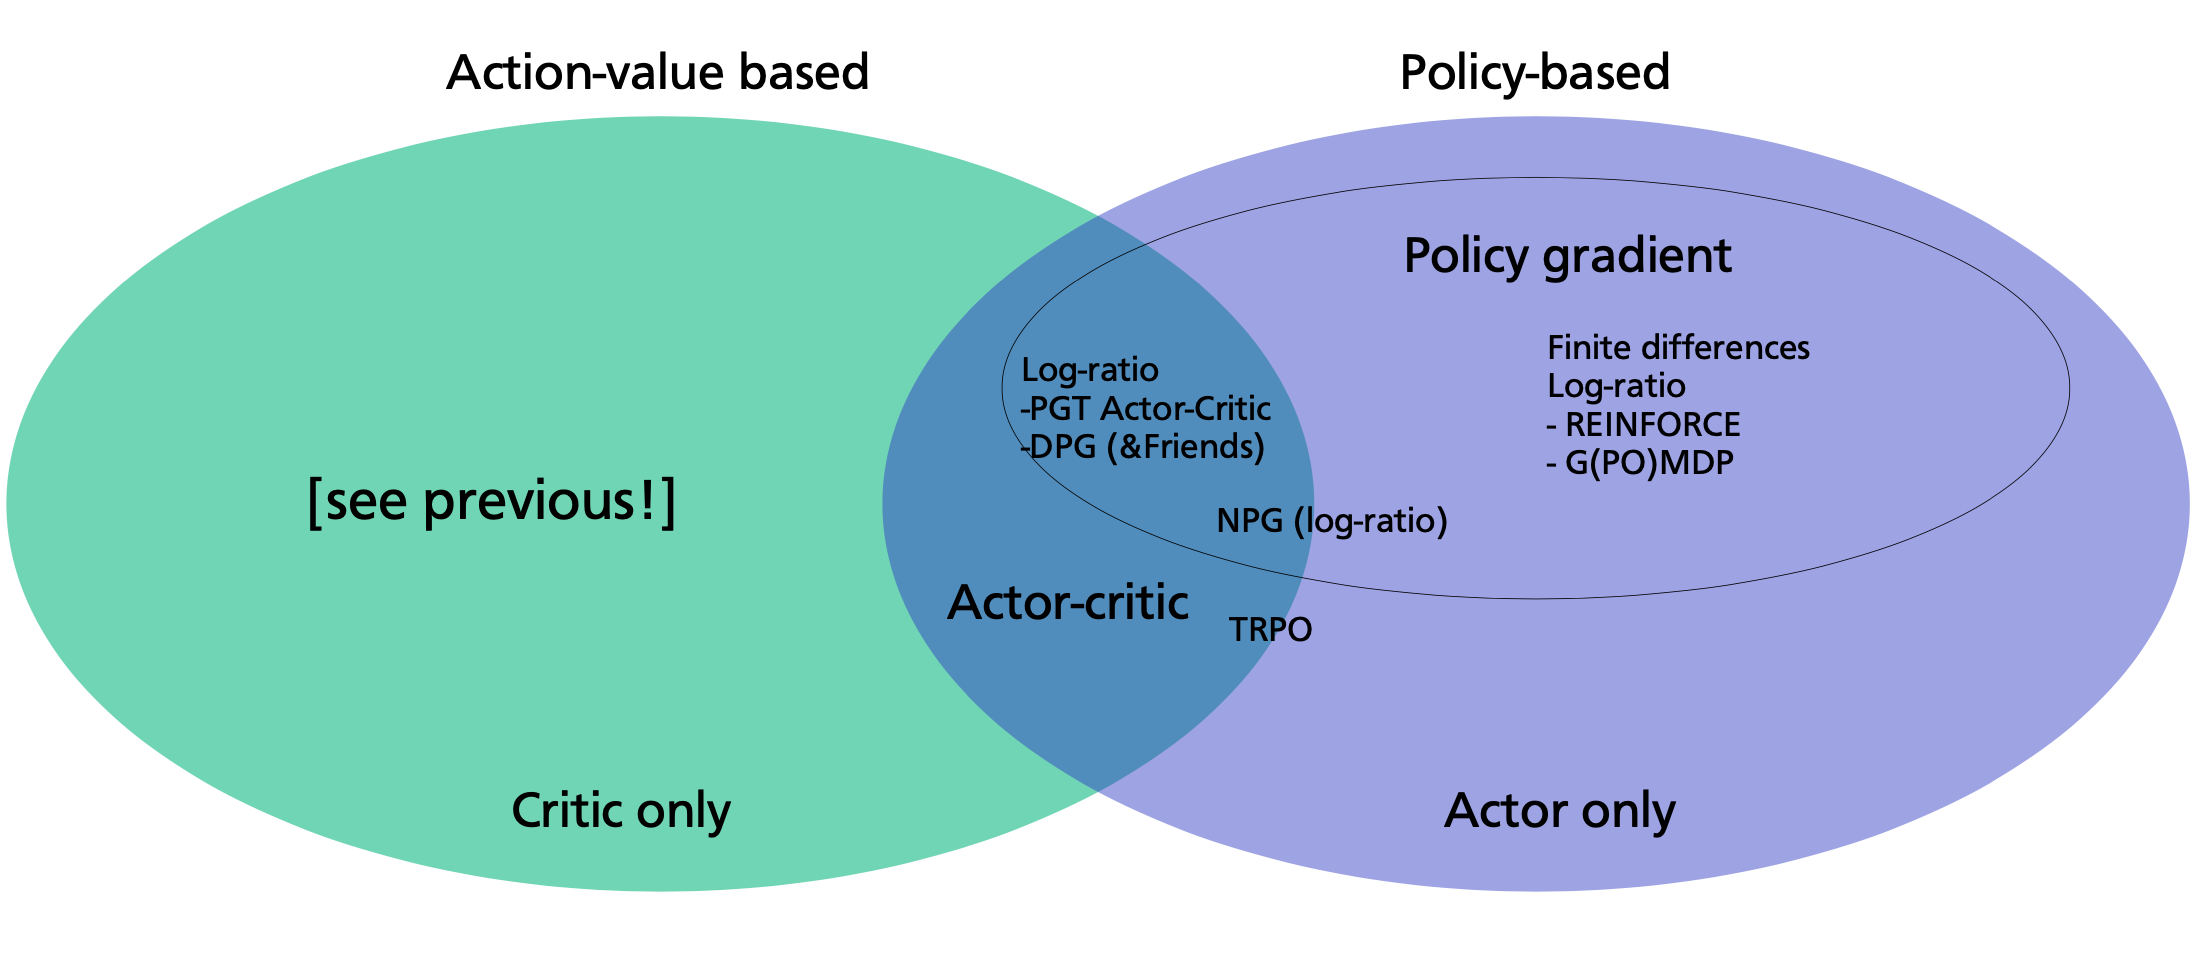
\includegraphics[width=\textwidth]{figures/rl_policy_gradient_summary_2.png}
			\caption{Actor-only versus Value-only methods}
		\end{subfigure}
		\caption{Comparing algorithms across two dimensions. (a) Pointing out the main difference between simple methods and advanced policy gradients (see text for more explanation). (b) Setting policy gradient methods into perspective with value-based.}
	\end{figure}

	\item When discussing the first algorithms of policy gradient, we could distinguish the methods on two dimensions:
	\begin{itemize}
		\item \textit{Exploration}: One key point in the discussion of PGPE was the exploration. Methods like REINFORCE explore by sampling an action at each time step independently, hence their exploration is step-based. PGPE however samples a new policy once in the beginning. This is episode-based because within the episode, we follow a deterministic policy and do not add noise per step. DDPG can be considered as in-between because it adds noise correlations between steps, and hence has not a purely step-based exploration strategy anymore. 
		
		In general, it is hard to say which of both is preferred, and possibly depends on the environment. Independent noise as in the step-based methods have been shown to explore worse (which is why DDPG added the correlation). However, PGPE is more complex to implement and to learn because we have to learn a distribution over parameters $\theta$ which do not one-to-one correspond to distribution over different policies (as discussed in NPG, relation between $\theta$ and $\pi$ might be quite complex).
		
		\item \textit{Evaluation}: Across our discussion, we have seen that some algorithms evaluate their actions step-wise and others per episode. We prefer methods that we can evaluate step-wise because they usually don't need a full sample until the end of an episode (except GPOMDP and other non-Actor-Critic methods), and give every step individual credit assignment. REINFORCE performs episode-based evaluations because the first steps reward influences the last steps update (which we tried to prevent in the other algorithms)
	\end{itemize}
	\item Another part is to consider the different sub-groups of policy-based methods with respect to value-based techniques. REINFORCE, G(PO)MDP and PGPE are all actor-only methods, meaning that they only learn a policy $\pi$. We have seen that we can extend most approaches by introducing a critic that learns $q_{\pi}(s,a)$.
	
	NPG and TRPO can be applied whether with or without actor-critic. Furthermore, we are free to choose how we arrive at $\nabla J$, but note that in the theoretical motivation of TRPO, we use the lower bound so that it is, strictly speaking, not a policy gradient method
\end{itemize}